\documentclass[11pt,a4paper]{article} 

\usepackage{titlesec}
\usepackage{color}
\usepackage[utf8]{inputenc}
\usepackage[english]{babel}
\usepackage[T1]{fontenc}
\usepackage{graphicx}
\graphicspath{{Images/}}
\usepackage{eso-pic} 
\usepackage{subfig} 
\usepackage{caption}
\usepackage{transparent}

% STANDARD MATH PACKAGES
\usepackage{amsmath}
\usepackage{amsthm}
\usepackage{bm}
\usepackage[overload]{empheq} 

% PACKAGES FOR TABLES
\usepackage{tabularx}
\usepackage{colortbl}

% PACKAGES FOR ALGORITHMS (PSEUDO-CODE)
\usepackage{algorithm}
\usepackage{algorithmic}

% PACKAGES FOR REFERENCES & BIBLIOGRAPHY
\usepackage[colorlinks=true,linkcolor=black,anchorcolor=black,citecolor=black,filecolor=black,menucolor=black,runcolor=black,urlcolor=black]{hyperref} % Adds clickable links at references
\usepackage{cleveref}
\usepackage[square, numbers, sort&compress]{natbib} 

\bibliographystyle{plain} % You may use a different style adapted to your field

% PACKAGES FOR THE APPENDIX
\usepackage{appendix}

% PACKAGES FOR ITEMIZE & ENUMERATES 
\usepackage{enumitem}

% OTHER PACKAGES
\usepackage{amsthm,thmtools,xcolor} % Coloured "Theorem"
\usepackage{fancyhdr} % Fancy headers and footers
\usepackage{lipsum} % Insert dummy text
\usepackage{tcolorbox} % Create coloured boxes


% Do not change Configuration_files/config.tex file unless you really know what you are doing.
%DO NOT EDIT
% Configuration package
\usepackage[bottom=2.0cm,top=2.0cm,left=2.0cm,right=2.0cm]{geometry}
\raggedbottom 

\definecolor{newblue}{cmyk}{0.4,0.1,0,0.4}

% Custom theorem environments
\declaretheoremstyle[
  headfont=\color{newblue}\normalfont\bfseries,
  bodyfont=\color{black}\normalfont\itshape,
]{colored}

\captionsetup[figure]{labelfont={color=newblue}} 
\captionsetup[table]{labelfont={color=newblue}} 
\captionsetup[algorithm]{labelfont={color=newblue}} 

\theoremstyle{colored}
\newtheorem{theorem}{Theorem}[section]
\newtheorem{proposition}{Proposition}[section]

\newcommand\T{\rule{0pt}{2.6ex}}
\newcommand\B{\rule[-1.2ex]{0pt}{0pt}}

\newcounter{algsubstate}
\renewcommand{\thealgsubstate}{\alph{algsubstate}}
\newenvironment{algsubstates}{
    \setcounter{algsubstate}{0}%
    \renewcommand{\STATE}{%
    \stepcounter{algsubstate}%
    \Statex {\small\thealgsubstate:}\space}
    }{}
    
% Custom theorem environment
\newcolumntype{L}[1]{>{\raggedright\let\newline\\\arraybackslash\hspace{0pt}}m{#1}}
\newcolumntype{C}[1]{>{\centering\let\newline\\\arraybackslash\hspace{0pt}}m{#1}}
\newcolumntype{R}[1]{>{\raggedleft\let\newline\\\arraybackslash\hspace{0pt}}m{#1}}

% Custom itemize environment
\setlist[itemize,1]{label=$\bullet$}
\setlist[itemize,2]{label=$\circ$}
\setlist[itemize,3]{label=$-$}
\setlist{nosep}


\setlength\parindent{0pt}

% Custom title commands
\titleformat{\section}
{\color{newblue}\normalfont\Large\bfseries}
{\color{newblue}\thesection.}{1em}{}
\titlespacing*{\section}
{0pt}{3.3ex}{3.3ex}

\titleformat{\subsection}
{\color{newblue}\normalfont\large\bfseries}
{\color{newblue}\thesubsection.}{1em}{}
\titlespacing*{\subsection}
{0pt}{3.3ex}{3.3ex}

% Custom headers and footers
\pagestyle{fancy}
\fancyhf{}
      
\fancyfoot{}
\fancyfoot[C]{\thepage} % page
\renewcommand{\headrulewidth}{0mm} % headrule width
\renewcommand{\footrulewidth}{0mm} % footrule width

\makeatletter
\patchcmd{\headrule}{\hrule}{\color{black}\hrule}{}{} % headrule
\patchcmd{\footrule}{\hrule}{\color{black}\hrule}{}{} % footrule
\makeatother

% Insert here the info that will be displayed into your Title page 
\renewcommand{\title}{Suffix Trees}
\newcommand{\authorA}{Aditya Patil (2021CSB1062)}
\newcommand{\authorB}{Alankrit Kadian (2021CSB1065)}
\newcommand{\authorC}{Harsh Raj Srivastava (2021CSB1091)} %comment if not needed
%\newcommand{\authorD}{Student4Name (ID4)} %comment if not needed
\newcommand{\advisor}{Dr. Anil Shukla}
\newcommand{\firstcoadvisor}{Akanksha}
\newcommand{\summary}{We have first performed and analysed the construction of the suffix tree in linear time using the \emph{Ukkonen's algorithm}. We also implemented our own thought application of suffix trees in which we also incorporated \emph{BK-Tree} and \emph{Bloom Filter}. In a encoded string we search a substring match and suggest the correct string if user input is wrong using BK-Tree from a unique set of keys defined by bloom filter and use suffix tree to finds all the occurences of the substring.}

%-------------------------------------------------------------------------
%	BEGIN OF YOUR DOCUMENT
%-------------------------------------------------------------------------
\begin{document}

% Do not change Configuration_files/TitlePage.tex
% DO NOT EDIT


\null\hfill
\includegraphics[width=0.2\textwidth]{Images/IIT_Rpr_logo.jpg}

\vspace{3mm}
\Large{\textbf{\color{newblue}{\title}}}
\vspace{0.1cm}\\
\null\hfill \today\\
\large{\textbf{\authorA}}\vspace{1mm}
,\\ \large{\textbf{\authorB}}\vspace{1mm}
\ifdefined \authorC
,\\ \large{\textbf{\authorC}}\vspace{1mm}
\ifdefined \authorD
,\\ \large{\textbf{\authorD}}\vspace{1mm}
\fi 
\fi
\small \normalfont

\vspace{11pt}

\centerline{\rule{1.0\textwidth}{0.4pt}}

\begin{center}
\begin{minipage}[t]{.24\textwidth}
\begin{minipage}{.90\textwidth}
\noindent
\footnotesize{\textbf{Instructor:} \\
\advisor} \\
\\
\footnotesize{\textbf{Teaching Assistant:}\\ 
\firstcoadvisor}\\ 

\end{minipage}
\end{minipage}
\begin{minipage}{.74\textwidth}
\noindent \textbf{\color{newblue} Summary:} {\summary}
\end{minipage}
\end{center}

\vspace{8pt}

\centerline{\rule{1.0\textwidth}{0.4pt}}
\vspace{12pt}
%Main Text starting point
\section{Introduction}
\label{sec:introduction}
A suffix tree is a data structure that exposes the internal structure of a string. Suffix trees are useful in various string processing and computational problems. They provide linear-time solutions to many complex string problems, after just O(m), or linear, preprocessing time of a given string. Applications of suffix trees include exact matching problem, substring problem, pattern searching, longest repeating substring, building linear time suffix array, longest common substring, longest palindromic substring, etc.

\section{Basic Introductions to Suffix Trees}
\label{sec:intro}
A suffix tree \begin{math}\tau\end{math} for an m-character string S is a rooted directed tree with exactly m leaves indexed 1 to m. For any leaf i, the concatenation of the edge-labels on the path from the root to leaf i exactly spells out the suffix of S that starts at position i, i.e. S[i...m]. Each internal node, other than the root, has at least two children and each edge is labeled with a non-empty substring of S. No two edges out of the same node can have edge-labels beginning with the same character.
\\
The \emph{label of a path} from the root that ends at a node is the concatenation in order, of the substrings labeling the edges of that path. The \emph{path label} of a node is the label of the path from the root to that node.
\\
For example, let us take a look at the suffix tree for string S = "xabxac" which have six suffixes, namely "xabxac", "abxac", "bxac", "xac, "ac" and "c".
\begin{figure}[H]
    \centering
    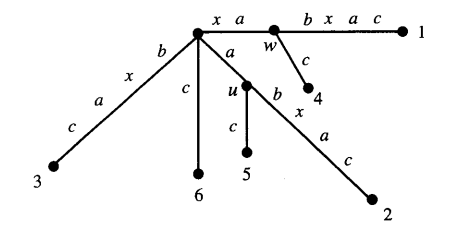
\includegraphics{Images/image1.png}
    \caption{Suffix Tree for string S = "xabxac"}
    \label{fig:suffixtreeExample}
\end{figure}
As shown in Figure 1, the suffix tree for string S has one root node, two internal nodes and six leaf edges representing each of its six suffixes.
\\
The above definition of a suffix tree for S does not gaurantee that the suffix tree for any string S actually exists. The problem is that if one suffix of S matches the prefix of another suffix of S, then no suffix tree obeying the above definition is possible. To avoid this problem, we have to assume that the last character of S appears nowhere else in S, so that no suffix of the resulting string can be a prefix of any other suffix. To achieve this in practice, we can add a character, like `\$', to the end of S that is not present in S already. This is called the \emph{termination character}. 

\section{Suffix Tree Construction}
There are various algorithms to build a suffix tree for a string S. First, we will present a straightforward algorithm which takes \begin{math}O(m^2)\end{math} time to build the suffix tree for a string S of length m, and then we will see another algorithm which, with some observations, tricks and implementation speedups, will build the suffix tree for us in linear i.e. \begin{math}O(m)\end{math} time.

\subsection{A naive algorithm to build a suffix tree}
\label{subsec:algorithm1}
This naive method first enters a single edge for suffix S[1...m]\$(the entire string) into the tree, and then it successively enters suffix S[i...m]\$ into the growing tree, for 2 $\le$ i $\le$ m. Let \begin{math}\tau\end{math}\textsubscript{i} denote the intermediate tree that encodes all the suffixes from 1 to i. 
\\
Tree \begin{math}\tau\end{math}\textsubscript{1} consists of a single edge between the root of the tree and a leaf labeled 1 and the edge is labeled with the string S\$. Tree \begin{math}\tau\end{math}\textsubscript{i+1} is constructed from \begin{math}\tau\end{math}\textsubscript{i} as follows:
\\
Starting at the root of \begin{math}\tau\end{math}\textsubscript{i}, find the longest path by successively comparing and matching characters from the root whose label matches a prefix of S[i+1...m]\$. The matching path will be unique as no two edges out of a node can have labels that begin with the same character. The matching path either ends at a node, say w, or it ends in the middle of an edge. If it is in the middle of an edge, say (u,v), then it breaks the edge (u,v) into edges by inserting in a new node, say w, just after the last character on that edge that mismatched. The new edge (u,w) is labeled with the part of (u,v) label that matched with S[i+1...m], and the new edge (w,v) is labeled with the remaining part of the (u,v) label. A new edge (w,i+1) running from w to a new leaf labeled i+1 is created, and it is labeled with the unmatched part of suffix S[i+1...m]\$. The suffix tree now contains a unique path from root to leaf i+1 with path label S[i+1...m]\$.
\\
As mentioned earlier, the naive method takes \begin{math}O(m^2)\end{math}
time to build a suffix tree for the string S of length m.

\subsection{Ukkonen's linear-time suffix tree algorithm}
\label{subsec:tables}
Esko Ukkonen devised a linear-time algorithm for constructing a suffix tree that, with its "on-line" property and the simplicity of its description, proof, and time analysis, may be the conceptually easiest linear-time construction algorithm. 
\\
While constructing suffix trees using Ukkonen's algorithm, we will see `implicit suffix tree' in some intermediate steps depending on characters in string S.
\\
An \emph{implicit suffix tree} for string S is a tree obtained from the suffix tree for S\$ by removing every copy of the termination character \$ from the edge labels of the tree, then removing any edge that has no label, and then removing any node that does not have two or more children. Even though an implicit suffix tree may not have a leaf for each suffix, it does encode all the suffixes of S, as each suffix is spelled out by the characters on some path from the root of the implicit suffix tree.

\subsection{Algorithms}
\label{subsec:algorithms}

Pseudo-algorithms can be written in \LaTeX{} with the \texttt{algorithm} and \texttt{algorithmic} packages.
An example is shown in Algorithm~\ref{alg:var}.
\begin{algorithm}[H]
\label{alg:example}
\caption{Name of the Algorithm}
\label{alg:var}
\label{protocol1}
\begin{algorithmic}[1]
\STATE Initial instructions
\FOR{$for-condition$}
\STATE{Some instructions}
\IF{$if-condition$}
\STATE{Some other instructions}
\ENDIF
\ENDFOR
\WHILE{$while-condition$}
\STATE{Some further instructions}
\ENDWHILE
\STATE Final instructions
\end{algorithmic}
\end{algorithm} 

\section{Some further useful suggestions}

Theorems have to be formatted as follows:
\begin{theorem}
\label{a_theorem}
Write here your theorem. 
\end{theorem}
\textit{Proof.} If useful you can report here the proof.
\vspace{0.3cm} % Insert vertical space

Propositions have to be formatted as follows:
\begin{proposition}
Write here your proposition.
\end{proposition}
\vspace{0.3cm} 

How to insert itemized lists:
\begin{itemize}
    \item first item;
    \item second item.
\end{itemize}
How to write numbered lists:
\begin{enumerate}
    \item first item;
    \item second item.
\end{enumerate}

\section{Conclusions}
\color{black}
A final section containing the main conclusions of your research/study
and possible future developments of your work have to be inserted in the section ``Conclusions''.

\section{Bibliography and citations}
Your thesis must contain a suitable Bibliography which lists all the sources consulted on developing the work.
The list of references is placed at the end of the manuscript after the chapter containing the conclusions.
It is suggested to use the BibTeX package and save the bibliographic references in the file \verb|bibliography.bib|.
This is indeed a database containing all the information about the references. To cite in your manuscript, use the \verb|\cite{}| command as follows:
\\
\textit{Here is how you cite bibliography entries: \cite{knuth74}, or multiple ones at once: \cite{knuth92,lamport94}}.
\\
The bibliography and list of references are generated automatically by running BibTeX \cite{bibtex}.

\section*{Acknowledgements}
Just before References, here you might want to acknowledge someone.

\bibliography{bibliography.bib}

\appendix
\section{Appendix A}
If you need to include an appendix to support the research in your thesis, you can place it at the end of the manuscript.
An appendix contains supplementary material (figures, tables, data, codes, mathematical proofs, surveys, \dots)
which supplement the main results contained in the previous sections.

\section{Appendix B}
It may be necessary to include another appendix to better organize the presentation of supplementary material.

\end{document}